\chapter{Ay Yerçekimi Modelleri ve Mascon Yaklaşımı}

% ============================================================
\section{Giriş}
\label{sec:introduction}

Ay, dış geometrisi itibarıyla Dünya ile kıyaslandığında şaşırtıcı bir biçimde ``daha küresel'' bir form sergiler. Dünya'nın hızlı rotasyonu sonucu oluşan belirgin ekvatoral şişkinliğin aksine, Ay'ın yavaş dönüş hızı ona geometrik bir mükemmelliğe çok daha yakın bir figür kazandırmıştır. Bu durum, iki gök cisminin basıklık oranları (\textit{flattening}) arasındaki belirgin fark ile gözlemlenebilir:
\[
f_{\text{Dünya}} \approx \frac{1}{298}
\quad \text{ve} \quad
f_{\text{Ay}} \approx \frac{1}{827}.
\]

Ancak bu geometrik sükunet, Ay'ın yerçekimi potansiyelindeki ekstrem heterojenlik ile keskin bir tezat oluşturur. Alçak Ay yörüngeleri (LLO -- \textit{Low Lunar Orbit}), Dünya çevresindeki benzerlerine kıyasla çok daha hırçın ve dinamik olarak kaotik bir doğaya sahiptir. Bu kararsızlığın temel kaynağı, Ay'ın soğuk ve rijit litosferinin, milyarlarca yıl boyunca yüzey altındaki devasa kütle dengesizliklerini (izostatik dengeden uzak yapıları) sönümlemeden günümüze kadar taşıyabilmiş olmasıdır.

\bigskip
Özellikle Ay'ın yakın yüzündeki (\textit{nearside}) geniş bazaltik denizler (\textit{mare}) ve devasa çarpma havzaları üzerinde seyreden uzay araçlarının Doppler hız verilerinde, ideal Keplerian yörünge modelinden sapan ani ve şiddetli ivmelenmeler rapor edilmiştir \cite{Muller1968}. 1960'ların sonunda keşfedilen ve ``mascon'' (\textit{mass concentration}) olarak adlandırılan bu kütle yoğunlaşmaları, Ay yerçekimi alanını sadece tek bir monopol (noktasal kütle) terimiyle temsil etmenin navigasyon ve yörünge kararlılığı açısından neden yetersiz kaldığını açıkça ortaya koymuştur \cite{Konopliv2001}. Görev tasarımı gereksinimlerinin gün geçtikçe hassaslaşması, Ay'ın bu ``pürüzlü'' yerçekimi imzasını yüksek dereceli küresel harmonik açılımlar ve \textit{Gravity Recovery and Interior Laboratory} (GRAIL) verilerine dayalı modern modellerle temsil etmeyi astrodinamik analizlerin vazgeçilmez bir unsuru haline getirmiştir \cite{Zuber2013}.


% ================ Ay Modellerinin Tarihçesi =====================
\newpage
\section{Ay Modellerinin Tarihçesi}

Ay yerçekimi modellerinin geliştirilmesi, hassas navigasyon ve yörünge kararlılığı gerektiren modern Ay görevleri için hayati öneme sahiptir. Basitleştirilmiş küresel modellerin sınırlılıkları erken Dünya görevlerinde fark edilmiş, Ay görevleriyle birlikte yapılan izleme ve ölçümler bu ihtiyacı belirginleştirerek daha yüksek doğruluklu modellerin geliştirilmesini hızlandırmıştır.


\paragraph{İlk Ay yörüngeleri: beklenmeyen pertürbasyonların ortaya çıkışı (1960'lar).}
Ay yörünge görevlerinin ilk dönemlerinde (1960’lar), uzay araçlarının yörünge elemanlarının zamanla beklenenden hızlı değiştiği; özellikle belirli bölgeler üzerinden geçişlerde belirgin hızlanma/yavaşlamalar oluştuğu rapor edilmiştir \cite{Muller1968}. Bu sapmaların ortak yönü, büyük çarpma havzaları ve mare alanlarıyla ilişkili görünmesidir. Bu dönemde öne çıkan sonuç şudur: Ay’ın yerçekimi alanındaki düzensizlikler ``küçük düzeltmeler'' seviyesinde değil, yörünge dinamiğini doğrudan belirleyecek kadar güçlü olabilir. Dolayısıyla Ay görevlerinde güvenilir propagasyon için, gravite alanının bölgesel anomalilerini
hesaba katan bir temsil gereklidir.

\paragraph{Mascon kavramı: fiziksel yorum ve modelleme fikri (1960'lar sonu--1970'ler başı).}
Bu pertürbasyonları açıklamak için literatürde \emph{mass concentration} terimi ortaya çıkmış ve kısaca \textbf{mascon} adıyla yerleşmiştir \cite{Muller1968}. Mascon kavramı, bazı büyük havzaların altında, çevresine göre daha yüksek etkin kütle (ya da yoğunluk) varmış gibi bir yerçekimi tepkisi doğduğunu ifade eder. Bu yaklaşımın kritik yanı, gözlenen sapmaları yalnızca ``ölçüm hatası'' veya ``model eksikliği'' olarak değil, Ay’ın jeolojik yapısı ve havzaların evrimiyle bağlantılı fiziksel bir gerçeklik olarak ele almasıdır. Böylece masconlar, hem yörünge dinamiği için bir pertürbasyon kaynağı hem de Ay içyapısını anlamak için
bir teşhis aracı hâline gelmiştir.

\paragraph{Apollo dönemi ve subsatelit takibi: nearside bilgisinin güçlenmesi (1970'ler).}
Apollo görevleri sırasında ve özellikle Apollo 15/16 ile ilişkilendirilen subsatelit takipleri,
Ay yerçekimi alanı hakkında daha uzun süreli ve daha hassas veri sağlamıştır. Bu dönem,
mascon etkisinin yalnızca birkaç noktada değil, geniş ölçekte yörüngeler üzerinde sistematik sonuçlar doğuran
bir yapı olduğunu daha net göstermiştir. Bununla birlikte temel bir kısıt da belirginleşmiştir:
Dünya’dan radyo takibi, Ay’ın uzak tarafında (farside) doğrudan görüş hattına sahip değildir.
Bu nedenle farside gravite alanı uzun süre görece belirsiz kalmış; model kalitesi nearside lehine
dengesizleşmiştir. Bu ``görüş hattı problemi'', Ay gravite modellemesinin tarihsel sınırlamalarından biridir.

\paragraph{Küresel temsile geçiş: sferik harmonik modellerin yaygınlaşması (1990'lar--2000'ler).}
1990’lar ve 2000’lerin başında daha uzun süreli ve daha iyi izlenen yörünge görevleri,
Ay gravite modellerinin iyileşmesini hızlandırmıştır. Bu dönemde öne çıkan eğilim,
yerçekimi alanının giderek daha yüksek derece/mertebede \textbf{sferik harmonikler} ile temsil edilmesidir.
Özellikle düşük irtifalı ve polar yörüngeler, kısa dalga boyu gravite bileşenlerine daha duyarlı oldukları için
katsayıların daha ileri seviyelere taşınmasına imkân vermiştir. Böylece yalnızca düşük dereceli (kaba) terimlerle yetinen
yaklaşımlar yerini çok terimli küresel modellere bırakmıştır.

\paragraph{Farside Belirsizliğinin Azalması: SELENE/Kaguya (2007--2010).} Japonya'nın SELENE (Kaguya) görevi, Ay'ın uzak yüzündeki (\textit{farside}) gravite alanının haritalanmasında tarihi bir kırılma noktası yaratmıştır. Bu görevin asıl başarısı, ana uydu uzak yüzün üzerindeyken Dünya ile olan iletişim kısıtını (görüş hattı problemi), bir röle uydu (\textit{Okina}) kullanarak gerçekleştirdiği dört yollu Doppler takibi (\textit{4-way Doppler tracking}) yöntemiyle aşmış olmasıdır. Bu teknik sayesinde, tarihte ilk kez Ay'ın uzak yüzünden doğrudan gravite verisi toplanabilmiş; \textit{nearside-farside} veri kalitesi arasındaki kronik dengesizlik giderilerek çok daha kararlı yörünge kestirimlerinin önü açılmıştır.

\paragraph{GRAIL ile Çözünürlük Sıçraması: Modern Ay Gravite Haritası (2011--2012).}
Ay gravite modellemesindeki en büyük kırılma noktası, \textit{Gravity Recovery and Interior Laboratory} (GRAIL) göreviyle gerçekleşmiştir. Önceki misyonların aksine GRAIL, yerden takip yerine uydudan uyduya mesafe ölçümü (\textit{Satellite-to-Satellite Tracking}) yöntemini kullanmış; ``Ebb'' ve ``Flow'' adlı iki ikiz uzay aracı arasındaki mesafe değişimlerini mikrometre hassasiyetinde ölçerek Ay'ın yerçekimi alanını eşsiz bir çözünürlükle haritalandırmıştır \cite{Zuber2013}. Bu misyon, sferik harmonik modellerin 420. derece ve üzerine (bazı güncel çözümlerde 1200. dereceye kadar) taşınmasını sağlayarak, Ay kabuğunun beklenenden çok daha gözenekli yapısını ve masconların detaylı morfolojisini ortaya koymuştur. GRAIL verileriyle birlikte Ay, Güneş Sistemi'nde yerçekimi alanı en hassas bilinen gök cismi haline gelmiştir.



\paragraph{Günümüz: Uygulamalı Astrodinamik ve Artemis Dönemi (2013--Günümüz).}
GRAIL sonrası dönem, teorik haritalama sürecinden ``yüksek hassasiyetli operasyonel uygulama'' safhasına geçişi temsil eder. Günümüzde GRGM1200A gibi ultra yüksek çözünürlüklü modeller, sadece bilimsel araştırmalarda değil, özellikle \textit{Artemis} programı kapsamındaki iniş görevlerinde kritik rol oynamaktadır. Modern astrodinamik çalışmaları artık bu devasa gravite veri setlerini, \textit{Lunar Reconnaissance Orbiter} (LRO) gibi görevlerden gelen lazer altimetri verileriyle birleştirerek; otonom iniş sistemleri, düşük irtifa yörünge kararlılığı ve \textit{Lunar Gateway} gibi istasyonlar için gerekli olan donmuş yörünge (\textit{frozen orbit}) tasarımlarında temel referans olarak kullanmaktadır. Bu süreçte Ay, bir keşif hedefinden öte, karmaşık perturbasyon modellerinin test edildiği yüksek sadakatli bir kütleçekim laboratuvarına dönüşmüştür.




% ============ Ay Topoğrafyası ve Kabuk Yapısı ============
\section{Ay Topoğrafyası ve Kabuk Jeofiziği}
\label{sec:moon_topography}

Ay topoğrafyası, Güneş Sistemi'nin erken dönemlerinden bugüne uzanan çarpma kayıtlarını ve volkanik evrimi aynı anda
taşıyan, belirgin biçimde heterojen bir yapı sergiler. Ay'ın Dünya'ya gelgit kilitli (eşzamanlı dönme,
\textit{synchronous rotation}) olması nedeniyle, Dünya'dan sürekli gördüğümüz yakın yan (\textit{nearside}) ile
uzak yan (\textit{farside}) arasında dikkat çekici bir topoğrafik fark bulunur: yakın yan geniş bazaltik düzlüklerle
(\textit{maria}) öne çıkarken, uzak yan daha çok yoğun kraterlenmiş yüksek arazilerden (\textit{highlands}) oluşur
\cite{Zuber2013}.

% ----------------- Yerçekimi ve Topografya -----------
\subsection{Yerçekimi ve Topoğrafya Korelasyonu}

Topoğrafyadaki bu belirgin farklılıkların, yerçekimi alanına nasıl yansıdığı Ay jeofiziğinin temel sorularından biridir.
Bu ilişkiyi ayrıntılı biçimde incelemek, ancak yüksek çözünürlüklü yerçekimi verileriyle mümkündür. GRAIL misyonu ile
Ay'ın yerçekimi alanı küresel harmoniklerde çok yüksek derecelere kadar modellenmiş ve bu sayede kilometre mertebesinde
ayrıntıları ayırt etmek mümkün hale gelmiştir \cite{Zuber2013}. Bu tür modellerin önemli bir sonucu şudur:
belirli bir ölçek aralığında yerçekimi sinyalinin büyük kısmı, yüzey topoğrafyasının beklenen etkisiyle uyumlu görünür.
Başka bir deyişle, yüzeydeki kabartı ve çukurluklar yalnızca şekil olarak değil, kütle dağılımı üzerinden yerçekimi
ölçümlerinde de güçlü bir iz bırakmaktadır \cite{Zuber2013}.

Bu noktada iki kavram özellikle işe yarar. İlki serbest hava (\textit{free-air}) anomalisi: yerçekimi ölçümlerinin
yükseklik/geometri etkileriyle birlikte görünen ham imzasını temsil eder. İkincisi Bouguer anomalisi: topoğrafyanın
kendi kütle çekimi etkisi çıkarıldıktan sonra geriye kalan ve daha çok yüzey altı yapılarla ilişkilendirilen bileşendir.
Dolayısıyla Bouguer anomalileri, örneğin kabuk kalınlığındaki değişimleri veya kabuk içindeki yoğunluk farklarını
daha doğrudan incelemek için kullanılır. Bu düzeltmeler yapılırken pratikte ortalama bir kabuk yoğunluğu kabul edilir;
Ay için yaygın kullanılan değerlerden biri $\rho \approx 2560~\text{kg m}^{-3}$ mertebesindedir \cite{Zuber2013}.


\subsection{Kütle Konsantrasyonları (Masconlar)}

Ay yerçekimi alanındaki en belirgin yerel özellikler, ilk kez Muller ve Sjogren (1968) tarafından tanımlanan kütle konsantrasyonları veya ``mascon'' yapılarıdır \cite{Muller1968,Zuber2013}. Bu yapılar, özellikle Imbrium, Serenitatis, Crisium, Nectaris ve Humorum gibi yakın yandaki büyük halkalı çarpma havzalarının altında gözlenen pozitif yerçekimi anomalileridir \cite{Muller1968}. Jeofiziksel yorum açısından bu pozitif anomali; (i) havza oluşumu sırasında kabuğun incelmesi ve daha yoğun derin malzemenin daha sığ derinliklere yaklaşması, (ii) daha sonraki evrelerde havzanın bazaltik lavlarla dolarak etkin yoğunluğun artması ve/veya (iii) havza altında manto yükselimi gibi süreçlerin bileşimiyle ilişkilendirilir \cite{Zuber2013}.

\textit{Lunar Prospector} (LP) misyonu, bu yapıların yalnızca yakın yanla sınırlı olmadığını; uzak yandaki bazı havzalarda da (ör.\ Korolev ve Moscoviense) mascon izlerinin bulunduğunu teyit etmiştir \cite{Konopliv2001}. GRAIL verileri ise masconların ince detaylarını; havza halkalarının yerçekimi imzalarını, merkezi yapıları ve havza altındaki kabuk incelmesiyle tutarlı uzun dalga bileşenlerini yüksek hassasiyetle ortaya koymuştur \cite{Zuber2013}.

\subsection{Sayısal Parametreler ve Kabuk Dinamiği}

Ay'ın yerçekimi potansiyeli ($U$), normalize edilmiş küresel harmonik açılımı ile şu şekilde ifade edilebilir \cite{Konopliv2001}:
\begin{equation}
U(r,\phi,\lambda) =
\frac{GM}{r}
\left[
1 + \sum_{\ell=2}^{\infty}\sum_{m=0}^{\ell}
\left(\frac{R_{ay}}{r}\right)^{\ell}
\bar{P}_{\ell}^m[\sin\phi]
\left(
\bar{C}_{\ell,m}\cos m\lambda + \bar{S}_{\ell,m}\sin m\lambda
\right)
\right],
\end{equation}
burada $R_{ay}$ referans yarıçapı (1738.0 km), $\ell$ derece ve $m$ sırayı temsil etmektedir \cite{Konopliv2001}. LP verileriyle hesaplanan normalize edilmiş polar atalet momenti $C/MR^2 = 0.3932 \pm 0.0002$ olarak belirlenmiş; bu sonuç Ay'ın metalik bir çekirdeğe sahip olduğu yönündeki kısıtlamaları güçlendirmiştir \cite{Konopliv2001}. Ayrıca, Ay'ın dinamik Love sayısı $k_2 \approx 0.026 \pm 0.003$ olarak tahmin edilerek iç yapının elastik tepkisi hakkında nicel bilgi sağlanmıştır \cite{Konopliv2001}.



%============== Ay Yüzey Morfolojisi ==================
\section{Ay Yüzey Morfolojisinin Karakteristikleri}\label{sec:lunar_morphology}

Önceki bölümde özetlenen topoğrafik dikotomi, Ay yüzeyinin farklı morfolojik birimlere ayrılmasını da belirginleştirmektedir. Ay yüzeyi, Dünya'daki gibi plaka tektoniği ve atmosferik/hidrosferik erozyon süreçleriyle sürekli olarak yeniden şekillenmediğinden, erken dönemlerden itibaren biriken çarpma izlerinin önemli bir kısmını günümüze kadar koruyabilmiştir. Bu nedenle Ay topoğrafyasındaki çeşitlilik; albedo farkları, yükseklik varyasyonları ve litolojik farklılıklar üzerinden Tablo~\ref{tab:lunar_features}'de özetlenen başlıca morfolojik birimlerle sınıflandırılabilir.

\medskip
Dünya okyanuslarının aksine, Ay'da bulunan \textit{Oceanus} ve \textit{Maria} bölgeleri sıvı su barındırmaz; bu yapılar, devasa çarpma havzalarının daha sonraki dönemlerde bazaltik lavlarla dolması sonucu oluşmuş geniş volkanik ovalardır. Tablo~\ref{tab:lunar_features}'de verilen \textit{Oceanus Procellarum}, bu birimlerin en geniş örneklerinden biridir. Ay'daki vadiler (\textit{vallis}) ve oluklar (\textit{rimae}) ise Dünya'daki akarsu erozyonu ile oluşmuş kanyonlardan kökensel olarak farklıdır. Bu yapılar çoğunlukla kabuksal gerilme altında gelişen graben sistemleri veya geçmiş volkanizma evrelerinde oluşan lav kanalı/tüpü morfolojileri ile açıklanmaktadır.



\begin{table}[htbp]
\centering
\small
\caption{Ay Yüzeyindeki Temel \textit{Maria}, \textit{Oceanus} ve \textit{Vallis} Yapıları}
\label{tab:lunar_features}

% Sütun tanımları: 
% >{\centering\arraybackslash} ifadesi her hücrenin içindeki metni ortalar.
\begin{tabularx}{\textwidth}{@{} 
    >{\centering\arraybackslash}p{2.5cm} 
    >{\centering\arraybackslash}p{4.2cm} 
    >{\centering\arraybackslash}c 
    >{\centering\arraybackslash}X @{}}
\toprule
\textbf{Yapı Türü} & \textbf{İsim} \newline {\footnotesize \textbf{(Latince / Türkçe)}} & \textbf{Koordinat} & \textbf{Özellik / Önem} \\ 
\midrule

\textbf{Okyanus} & \textit{Oceanus Procellarum} \newline {\footnotesize (Fırtınalar Okyanusu)} & $26^{\circ}\text{N}, 49^{\circ}\text{W}$ & Ay'ın en geniş mare bölgesidir; karmaşık volkanik geçmişe sahiptir. \\ 

\midrule

\textbf{Deniz} & \textit{Mare Imbrium} \newline {\footnotesize (Yağmurlar Denizi)} & $32^{\circ}\text{N}, 15^{\circ}\text{W}$ & Belirgin mascon yapısı; yörünge perturbasyonları için kritiktir. \\ 
\addlinespace
& \textit{Mare Serenitatis} \newline {\footnotesize (Huzur Denizi)} & $28^{\circ}\text{N}, 17^{\circ}\text{E}$ & Apollo 17 iniş sahası; yüksek titanyum içerikli bazaltlar barındırır. \\ 
\addlinespace
& \textit{Mare Tranquillitatis} \newline {\footnotesize (Sessizlik Denizi)} & $8^{\circ}\text{N}, 31^{\circ}\text{E}$ & Apollo 11'in iniş yaptığı tarihsel bölgedir. \\ 
\addlinespace
& \textit{Mare Crisium} \newline {\footnotesize (Bunalımlar Denizi)} & $17^{\circ}\text{N}, 59^{\circ}\text{E}$ & Dairesel havza yapısı ile yerçekimi modelleme çalışmalarında referanstır. \\ 
\addlinespace
& \textit{Mare Nectaris} \newline {\footnotesize (Nektar Denizi)} & $15^{\circ}\text{S}, 35^{\circ}\text{E}$ & Çok halkalı çarpma havzalarının evrimini temsil eder. \\ 
\addlinespace
& \textit{Mare Orientale} \newline {\footnotesize (Doğu Denizi)} & $19^{\circ}\text{S}, 92^{\circ}\text{W}$ & Ay'ın en genç ve iyi korunmuş çok halkalı havzalarındandır. \\ 

\midrule

\textbf{Vadi / Oluk} & \textit{Vallis Alpes} \newline {\footnotesize (Alp Vadisi)} & $48^{\circ}\text{N}, 3^{\circ}\text{E}$ & $\sim$166 km uzunluğunda; kabuksal gerilme ile ilişkili bir graben sistemi. \\ 
\addlinespace
& \textit{Vallis Schröteri} \newline {\footnotesize (Schröter Vadisi)} & $26^{\circ}\text{N}, 51^{\circ}\text{W}$ & Ay'daki en geniş kıvrımlı oluk örneğidir; lav akışlarıyla ilişkilidir. \\ 
\addlinespace
& \textit{Rima Hadley} \newline {\footnotesize (Hadley Oluğu)} & $25^{\circ}\text{N}, 3^{\circ}\text{E}$ & Apollo 15 bölgesinde yer alan, volkanik süreçlerle oluşmuş kanal. \\ 

\bottomrule
\end{tabularx}
\end{table}


Ay'ın yerçekimi alanı, Dünya'ya kıyasla belirgin biçimde daha heterojendir. Dünya'da topoğrafik yüklerin önemli bir
kısmı, astenosferik akış ve izostatik denge mekanizmaları sayesinde jeolojik zaman ölçeklerinde kısmen dengelenir ve
yerçekimi imzası görece ``yumuşatılır''. Ay'da ise kalın ve soğuk litosfer, bu tür yeniden dengelenme süreçlerini daha
sınırlı ölçekte mümkün kıldığı için, mascon olarak adlandırılan kütle konsantrasyonları uzun zaman boyunca korunabilmiştir
\cite{Zuber2013}. Bunun sonucu olarak Ay çevresindeki alçak irtifa yörüngeleri, kısa dalga boylu yerçekimi
pertürbasyonlarının baskın olduğu ve yörünge kararlılığının hassas biçimde modellenmesini gerektiren daha ``sert''
bir dinamik ortam sunar.

Topoğrafya ve kabuk jeofiziği birlikte ele alındığında, Ay yerçekimi alanındaki yerel heterojenliklerin yalnızca yüzey
şekilleriyle açıklanmadığı görülür. Kabuk kalınlığındaki bölgesel değişimler, yoğunluk dağılımındaki kontrastlar ve
özellikle havza ölçekli iç yapı farklılıkları, yerçekimi anomalilerinin büyüklüğünü ve uzaysal desenini belirgin biçimde
etkiler. Bu bağlamda, büyük çarpma havzalarının altında gözlenen pozitif yerçekimi anomalileri ayrı bir önem taşır:
bu anomaliler alçak irtifa Ay yörüngelerinde ölçülebilir pertürbasyonlar üretir ve ilgili bölgeleri hem jeofiziksel yorumlar
hem de yörünge dinamiği açısından kritik hale getirir. Literatürde bu tür yerel kütle yoğunlaşmalarını tanımlamak ve
temsil etmek için kullanılan \textit{mascon} kavramı, bir sonraki bölümde hem fiziksel anlamı hem de yerçekimi alanı
modellemesindeki rolü açısından ayrıntılı olarak incelenecektir.




% ============= Mascon Teriminin İki Kullanımı ==============
\section{Mascon Nedir?}
\label{sec:mascon_def}

Mascon (\emph{mass concentration}) terimi, Ay yörüngesindeki uzay araçlarının hareketlerinde
gözlenen beklenmedik pertürbasyonları açıklamak üzere literatüre, Muller ve Sjogren tarafından
1968 yılında kazandırılmıştır \cite{Muller1968}. Özellikle mare bölgeleri ve büyük çarpma havzaları
üzerinde ölçülen belirgin pozitif yerçekimi anomalileri, bu bölgelerde çevresine kıyasla daha yoğun
bir kütle dağılımı bulunduğunu ima eder; bu tür anomali kaynaklı bölgeler zamanla ``mascon'' olarak
adlandırılmıştır. Daha sonra yüksek çözünürlüklü gravite alanı çözümlerinin gelişmesiyle birlikte
``mascon'' sözcüğü yalnızca fiziksel anomalileri değil, aynı zamanda bu anomalileri temsil etmeye
yönelik \textbf{yerel parametrizasyonları} da ifade edecek şekilde çift anlamlı bir kullanım kazanmıştır.
Aşağıda bu iki kullanım ayrımı verilmiştir.

Literatürde mascon terimi iki farklı anlamda kullanılır ve bu ayrım, Ay yerçekimi alanını hangi temsil
ile modelleyeceğimizi tartışırken açıklık sağlar.

\paragraph{(i) Fiziksel mascon (anomali).}
Bu kullanımda mascon, Ay'da gerçekten var olan bir yerçekimi anomalisi anlamına gelir. Örneğin belirli bir mare
veya çarpma havzası üzerinde ölçülen pozitif yerçekimi anomalisi ``mascon bölgesi'' olarak adlandırılır.
Burada vurgu, yörüngelerde gözlenen pertürbasyonun kaynağının yüzey/alt-yapı ile ilişkili fiziksel bir kütle
dağılımı olmasına yöneliktir.

\paragraph{(ii) Mascon modeli (temsil yaklaşımı).}
Bu kullanımda mascon, yerçekimi alanını temsil etmek için seçilen parametrizasyonu ifade eder.
Küresel harmoniklerde alan, tüm yüzeye yayılmış küresel baz fonksiyonlarıyla açılırken; mascon yaklaşımında alan,
yerel elemanlar veya baz fonksiyonları üzerinden yazılır. Tipik bir gösterim
\[
\Delta U(\mathbf r)\;\approx\;\sum_{k=1}^{K} \mu_k\,\Psi_k(\mathbf r)
\]
şeklindedir; burada $\Psi_k$ yerel yamayı/baz fonksiyonunu (veya eşdeğer kütle elemanını), $\mu_k$ ise ilgili bölgenin
``etkin kütle'' parametresini temsil eder. Uygulamada masconlar grid hücreleri, yamalar veya bölgesel kütle elemanları
olarak tanımlanabilir. (Gerekli olduğunda ivme alanı, $\mathbf a=-\nabla U$ bağıntısı üzerinden elde edilir.)

Bu temsil, özellikle veri kapsamasının heterojen olduğu bölgelerde (tarihsel olarak uzak yan \textit{farside}),
yerel kısa dalga boylu ayrıntıların önemli olduğu düşük irtifa yörüngelerinde ve ters çözümün daha kararlı yapılmasının
gerektiği durumlarda öne çıkar.




% ================= Mascon Yaklaşımı ========================
\subsection{Ay Yerçekimi Modellemesinde Mascon Yaklaşımı}

Ay’ın yerçekim alanı, Dünya’ya kıyasla daha ``yerel ve güçlü'' anomalilerle donatılmıştır. Bu nedenle temsil seçimi yalnızca matematiksel bir tercih değil; irtifa, veri geometrisi ve görev hedefiyle doğrudan ilişkilidir.

\paragraph{Yerel anomaliler ve çözünürlük.}
Sferik harmonik açılım küresel bir baz kullanır: tek bir katsayı, tüm yüzeyde tanımlıdır.
Bu yüzden yerel bir anomali (örneğin belirli bir mascon havzası) sferik harmonik uzayında çok sayıda
yüksek derece terime ``dağılarak'' temsil edilir. Ay’da düşük irtifada uçuluyorsa kısa dalga boyu etkiler baskın hâle gelir
ve yalnızca sferik harmoniklerle aynı yerel ayrıntıyı yakalamak için derece/mertebenin ciddi biçimde büyümesi gerekir.
Mascon yaklaşımı ise anomaliyi doğrudan yerelleştirir; pratikte daha az parametreyle aynı bölgesel etkiyi
yakalamak mümkün olabilir.

\paragraph{Veri geometrisi ve gözlenebilirlik.}
Ay yerçekim alanı, uzay aracı izleme ölçümlerinden (Doppler, menzil, menzil-hızı vb.) ters problem olarak kestirilir.
Bu ölçümler uzay aracının geçtiği yörünge boyunca güçlü bilgi üretir; geçilmeyen bölgeler ise dolaylı kısıtlanır.
Tarihsel olarak farside tarafının zayıf gözlenmesi bu açıdan tipik bir örnektir.
Sferik harmonik katsayıları küresel olduğundan, zayıf veri bölgeleri katsayı uzayında daha yaygın belirsizliklere yol açabilir.
Mascon parametrizasyonu, çözümü daha yerel tuttuğu için veri kapsamasındaki heterojenliği daha ``doğrudan''
yansıtabilir; iyi gözlenen bölgelerde daha güçlü, zayıf bölgelerde daha kontrollü çözümler üretmeye elverişlidir.

\paragraph{Ters problem kararlılığı ve düzenlileştirme.}
Yüksek boyutlu gravite kestirimi ölçüm hataları ve veri eksikliği altında kararsızlaşabilir.
Sferik harmonik modellerde bu genellikle dereceye bağlı sönümleme veya apriori spektrum varsayımlarıyla yönetilir.
Mascon modellerinde ise komşu bölgeler arasında yumuşaklık/düzgünlük koşulları gibi daha sezgisel düzenlileştirmeler
kullanılabilir. Bu, özellikle düşük irtifada uzun süreli propagasyonlarda sayısal kararlılık açısından önemlidir.

\paragraph{Pratik kullanım alanları.}
Ay gravite modelleri doğrudan operasyonel hesaplara girer: (i) yörünge propagasyonu ve uzun dönem kararlılık analizi,
(ii) manevra planlama ve çarpma riskinin öngörülmesi, (iii) iniş/navigasyon problemlerinde hassas konumlama ve
ivme hata bütçesi. Düşük irtifa bilim görevlerinde kısa dalga boyu etkiler daha belirgin olduğundan,
yüksek dereceli sferik harmonikler veya mascon tabanlı temsiller kritik hâle gelir.
Cislunar görevlerde ve NRHO gibi yörüngelerde ise küçük gravite hataları uzun zaman ölçeklerinde faz hatasına
dönüşebildiği için, ``iyi düzenlileştirilmiş'' ve görev geometrisiyle uyumlu bir temsil seçimi önem kazanır.

\paragraph{Sonuç.}
Sferik harmonikler, küresel ölçekte tutarlı, standart ve analitik olarak ``temiz'' bir çerçeve sunduğu için
karşılaştırma ve raporlama açısından güçlü bir referans temsildir. Buna karşılık mascon yaklaşımı, Ay gibi yerel anomalilerin
baskın olduğu ortamlarda pertürbasyonları doğrudan uzaysal olarak yerelleştirerek; düşük irtifa propagasyonunda kritik olan
kısa dalga boyu bileşenleri daha etkin yakalayabilir ve heterojen veri kapsamasının etkilerini daha kontrollü biçimde yönetebilir.
Bu nedenle modern uygulamalarda iki temsil çoğu zaman rakip değil, farklı görev gereksinimlerine hizmet eden tamamlayıcı araçlar
olarak ele alınır; seçim, görev geometrisi ve hata bütçesi ile gerekirse çapraz doğrulama ihtiyacına göre yapılır.



% =============== Ayda Frozen Yörüngeler ==============
\section{Ayda Frozen Yörüngeler}
\label{sec:frozen_orbits}


Donmuş (\emph{frozen}) yörüngeler, seçilen bazı yörünge elemanlarının (en yaygın olarak dışmerkezlik $e$ ve enberi argümanı $\omega$) uzun zaman ölçeklerinde seküler olarak değişmediği, başka bir deyişle ortalama türevlerinin sıfıra yakın olduğu yörüngeler olarak tanımlanır. Dünya için \ref{sec:special_orbits} bölümünde incelenen Güneş-eşzamanlı, Molniya ve Tundra gibi yörüngeler bu fikre yakın örnekler sunar. Daha genel bir bakışla, ``zamana göre yaklaşık sabit kalan elemanlar kümesi'' seçilerek donmuş yörünge kavramı farklı görev ihtiyaçlarına göre genişletilebilir.

İlk bakışta Dünya çevresinde kullanılan analitik donmuş yörünge yaklaşımlarının Ay için de benzer şekilde uygulanabileceği düşünülebilir. Ancak Dünya'da bozunumların baskın kaynağı ekvatoral şişkinlik olduğundan, düşük dereceli zonal terimler (yaklaşık $J_2$--$J_5$) çoğu durumda perturbasyonların ana karakterini yeterli doğrulukla temsil eder. Ay'da ise yerçekimi alanındaki düzensizliklerin önemli bir kısmı mascon kökenli, kısa dalga boylu anomalilerden kaynaklandığı için yalnızca düşük dereceli zonal terimlerle yapılan modelleme, donmuş yörünge koşullarını yakalamakta genellikle yetersiz kalır. Bu nedenle Ay için donmuş yörünge analizi çoğu zaman daha yüksek dereceli yerçekimi modelleri ve sayısal entegrasyon ile desteklenir.

\subsection{Klasik Analitik Yaklaşımın (Seküler) Donma Koşulları}

Folta \& Quinn (2006) tarafından verilen seküler türev denklemleri \cite{Folta2006}, üçüncü-cisim etkisi benzeri bir form altında aşağıdaki şekilde yazılabilir:\footnote{Burada $n$ ortalama hareketi, $n_3$ ise ilgili pertürbatif ölçek frekansını temsil eder. Notasyon ve tanımlar çalışmanın ilgili kısmıyla tutarlı olacak biçimde verilmelidir.}

\begin{equation}
\label{eq:fq_set}
\begin{aligned}
\makebox[4.8cm][l]{\text{Yarı-büyük eksen:}} &
\frac{da}{dt} = 0, \\[3pt]
\makebox[4.8cm][l]{\text{Dışmerkezlik:}} &
\frac{de}{dt} = \frac{15}{8}\frac{n_{3}^{2}}{n}\, e \sqrt{1-e^{2}} \,\sin^{2} i \,\sin 2\omega, \\[3pt]
\makebox[4.8cm][l]{\text{Eğiklik:}} &
\frac{di}{dt} = -\frac{15}{16}\frac{n_{3}^{2}}{n}\,\frac{e^{2}}{\sqrt{1-e^{2}}}\,\sin 2i\, \sin 2\omega, \\[3pt]
\makebox[4.8cm][l]{\text{Çıkan düğüm boylamı:}} &
\frac{d\Omega}{dt} = \frac{3}{8}\frac{n_{3}^{2}}{n}\,\frac{\cos i}{\sqrt{1-e^{2}}}
\left( 5e^{2}\cos 2\omega - 3e^{2} - 2 \right), \\[3pt]
\makebox[4.8cm][l]{\text{Enberi argümanı:}} &
\frac{d\omega}{dt} = \frac{3}{16}\frac{n_{3}^{2}}{n}\,\frac{1}{\sqrt{1-e^{2}}}
\left[ (3+2e^{2}+5\cos 2i) + 5(1-2e^{2}-\cos 2i)\cos 2\omega \right].
\end{aligned}
\end{equation}


Bir ``donma'' koşulu aradığımızda temel hedef, seçilen eleman(lar) için seküler türevleri sıfıra (veya sıfıra çok yakın)
değerlere getirmektir. Literatürde en yaygın seçim, özellikle dışmerkezlik $e$ ile enberi argümanı $\omega$ elemanlarının
uzun dönem davranışını mümkün olduğunca sabitlemektir \cite{Folta2006}. Bu amaçla aşağıdaki iki koşul birlikte incelenir:
\begin{equation}
\label{eq:freeze_conditions}
\frac{de}{dt}=0,
\qquad
\frac{d\omega}{dt}=0.
\end{equation}

\paragraph{Adım 1: $\boldsymbol{de/dt=0}$ koşulu.}
\eqref{eq:fq_set} içindeki $de/dt$ ifadesi
\begin{equation}
\frac{de}{dt} \propto e\,\sin^{2}i\,\sin 2\omega
\end{equation}
şeklinde bir bağımlılığa sahip olduğundan, $de/dt=0$ için (aşikar \emph{trivial} olmayan çözümler haricinde) aşağıdaki olasılıklar elde edilir:
\begin{align}
e=0 \quad &(\text{dairesel yörünge}), \label{eq:cond_e0}\\
\sin i = 0 \;\Rightarrow\; i=0^\circ \text{ veya } 180^\circ \quad &(\text{ekvatoryal yörünge}), \label{eq:cond_i0}\\
\sin 2\omega=0 \;\Rightarrow\; \omega=0^\circ,\,90^\circ,\,180^\circ,\,270^\circ. \label{eq:cond_omega}
\end{align}

Dairesel ($e=0$) ve ekvatoryal ($i=0^\circ$) çözümler matematiksel olarak mümkün olsa da, Ay için pratik donmuş yörünge
tasarımlarında çoğunlukla $\omega$ seçimi üzerinden bir ``aile'' araştırılır. Bunun iki temel nedeni vardır:
(i) Ay çevresinde mascon kaynaklı kısa dalga boylu etkiler, $e$ ve özellikle perilune geometrisi üzerinde belirgin
sonuçlar doğurur; bu nedenle küçük fakat sıfır olmayan $e$ değerleri, model duyarlılığını artırdığı için tercih edilir.
(ii) $\omega$ ise periapsisin uzayda hangi doğrultuya ``baktığını'' belirlediğinden, mascon anomalilerinin boylamsal
yerleşimiyle etkileşimi doğrudan kontrol eden en etkili tasarım parametrelerinden biridir. Bu sebeple pratikte $e$'yi
sıfıra zorlamak yerine, $\omega$ üzerinden uygun denge yönelimleri seçilip $e$'nin seküler büyümesi bastırılmaya çalışılır.

\paragraph{Adım 2: $\boldsymbol{d\omega/dt=0}$ koşulu.}
\eqref{eq:fq_set} içindeki $d\omega/dt$ ifadesi sıfıra eşitlendiğinde, $\omega$ için kapalı-form ayrık çözümler elde etmek
genellikle kolay değildir. Bu nedenle yaygın yaklaşım, önce \eqref{eq:cond_omega} ile gelen aday $\omega$ değerlerini
yerine koyup $i$--$e$ ilişkisini incelemektir. Özellikle Ay uygulamalarında $\omega=90^\circ$ veya $270^\circ$ seçimleri
sıkça öne çıkar; çünkü bu yönelimler hem $\dot e$ koşulunu otomatik olarak sağlayan simetrik konumlar sunar, hem de
bazı konfigürasyonlarda perilune çevresindeki kütle anomalilerinin etkisini birbirini kısmen sönümleyecek şekilde
``fazlar'' (yani seküler sürüklenmeyi azaltma eğilimi gösterir).

\eqref{eq:cond_omega} içinden
\begin{equation}
\omega=90^\circ \ \text{veya}\ 270^\circ
\quad\Rightarrow\quad
\cos 2\omega = -1
\end{equation}
seçimi yapıldığında, cebirsel sadeleştirme sonucunda şu formda bir bağıntı elde edilir:
\begin{equation}
\label{eq:e_i_relation}
e = \left( 1 - \frac{5}{3}\cos^{2} i \right)^{1/2}.
\end{equation}

\paragraph{Gerçel çözüm koşulu ve kritik eğiklik.}
\eqref{eq:e_i_relation} ifadesinin gerçel (fiziksel) bir dışmerkezlik üretmesi için kök içinin negatif olmaması gerekir:
\begin{align}
1 - \frac{5}{3}\cos^{2} i \ge 0
\quad &\Rightarrow \quad
\cos^{2} i \le \frac{3}{5}
\quad \Rightarrow \quad
| \cos i | \le \sqrt{\frac{3}{5}}.
\end{align}
Buna karşılık gelen kritik eğiklik
\begin{equation}
\label{eq:icrit}
i \ge \cos^{-1}\!\left(\sqrt{\frac{3}{5}}\right)
\approx 39.23^\circ
\end{equation}
olarak bulunur. Dolayısıyla bu analitik model altında, \eqref{eq:e_i_relation} ile tanımlanan donmuş yörünge ailesi yalnızca
$i \gtrsim 39.23^\circ$ için gerçel dışmerkezlik ($e$) değerleri üretmektedir. Bununla birlikte, bu bulgu $i<39.23^\circ$
bölgesinde ``donmuş yörünge mümkün değildir'' şeklinde yorumlanmamalıdır. Burada elde edilen kritik eğiklik, kullanılan düşük
mertebeden ve idealize edilmiş seküler yaklaşımın bu aralıkta kapalı-form (analitik) bir denge çözümü vermediğini gösterir.
Ay yerçekimi alanındaki mascon kökenli kısa dalga boylu pertürbasyonlar dikkate alındığında, donmuş yörünge karakteristiğinin
daha gerçekçi biçimde değerlendirilmesi için yüksek dereceli küresel harmonik yerçekimi modelleri ile sayısal entegrasyon
(ör.\ Cowell) analizleri gereklidir.


\begin{figure}[h]
    \centering
    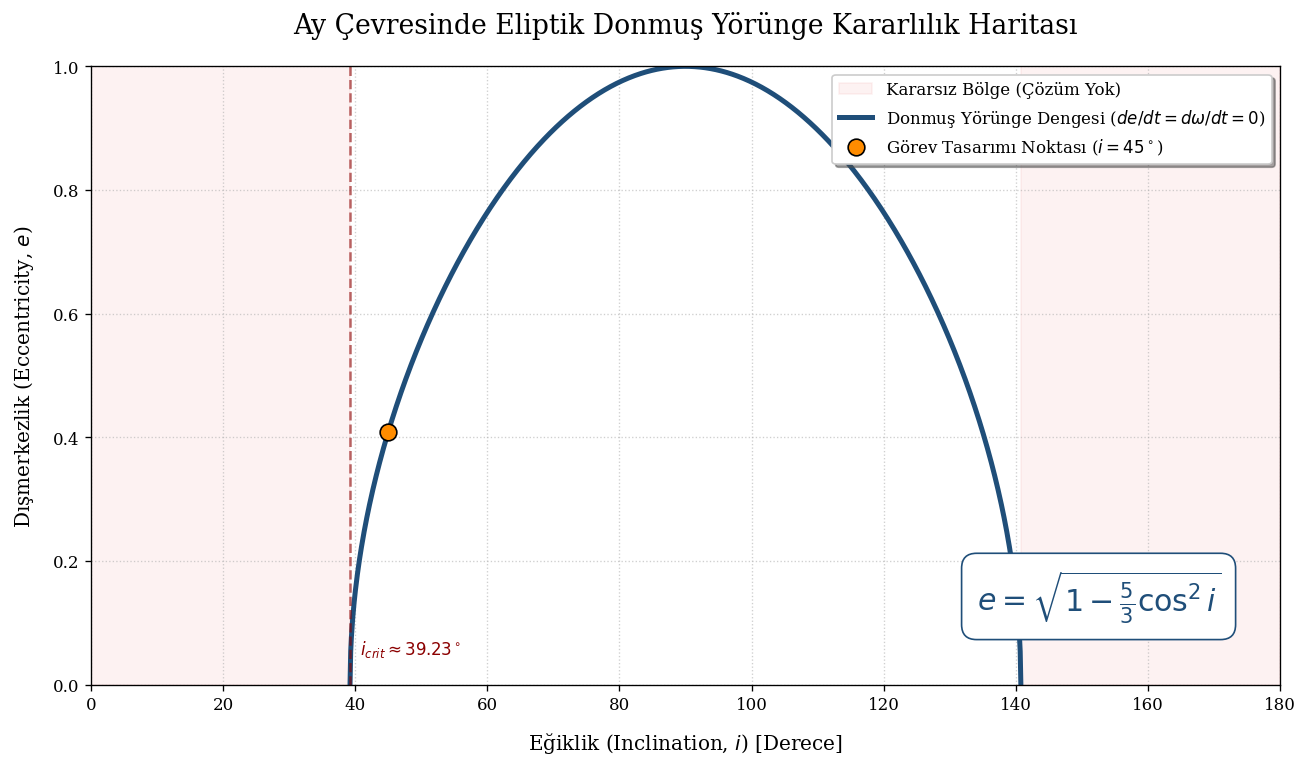
\includegraphics[width=0.92\linewidth]{Resimler/Ay Modeli/Frozen Orbit.png}
    \caption{Ay çevresinde eliptik donmuş yörünge denge eğrisi: $\dot{e}=0$ ve $\dot{\omega}=0$ koşullarını sağlayan
    analitik çözüm ailesi ve kritik eğiklik ($i_{\mathrm{crit}}\approx 39.23^\circ$) bölgesi.}
    \label{fig:frozen_orbit_map}
\end{figure}


Frozen testinin ayırt edici olabilmesi için seçilen yörünge, (i) kısa dalga boylu yerçekimi içeriğini
(har.\ yüksek derece terimleri / mascon etkileri) dinamiğe yeterince yansıtacak kadar ``hassas'',
ancak (ii) topografya kaynaklı çarpışma riski ve integratör hatalarını büyütecek kadar da ``aşırı agresif''
olmayacak şekilde seçilmelidir. Bu dengeyi sağlamak için başlangıç koşulları çoğunlukla aşağıdaki ilkelerle belirlenir:

\begin{itemize}
\item \textbf{Alçak irtifa (yaklaşık 20--60 km perilune yüksekliği):}
yüksek dereceli (kısa dalga boylu) bileşenleri belirginleştirerek mascon kaynaklı yerel anomalilerin
yörünge elemanlarına etkisini görünür kılar. (Bu aralık aynı zamanda topografya nedeniyle emniyet marjı gerektirir.)
\item \textbf{Küçük--orta dışmerkezlik ($e\simeq 0.01$--$0.05$):}
perilune civarında duyarlılığı artırır; buna karşın yüksek $e$ durumlarında görülen ``sertleşme''
(çok farklı zaman ölçekleri / adım-boyu hassasiyeti) etkilerini sınırlı tutarak sayısal kararlılığı korur.
\item \textbf{Polar/polar-yakın eğiklik ($i\approx 90^\circ$):}
geniş kapsama sağlayarak yerel anomalilerin farklı boylamlarda örneklenmesini kolaylaştırır ve
temsil hatalarını ``küresel tarama'' üzerinden ayırt etmeye yardım eder.
\item \textbf{Başlangıç enberi argümanı ($\omega$):}
$\omega=90^\circ$ veya $270^\circ$ seçimleri, analitik donma koşullarında sık çıkan simetrilerle uyumu ve
pratikte bazı konfigürasyonlarda seküler sürüklenmeleri azaltma eğilimi nedeniyle test başlangıcı için kullanışlıdır.
\end{itemize}

\paragraph{Örnek başlangıç parametreleri (temsilî).}
Aşağıdaki örnek, tek bir ``standart'' yörünge önermekten ziyade, testin duyarlılık aralığını
temsil eden tipik bir başlangıç kümesini göstermektedir.

\begin{table}[htbp]
\centering
\caption{Temsilî frozen-test başlangıç yörüngesi (Ay merkezli Kepler elemanları).}
\label{tab:frozen_test_ic}
\small
\begin{tabular}{l c c p{7.2cm}}
\toprule
\textbf{Büyüklük} & \textbf{Sembol} & \textbf{Değer} & \textbf{Not} \\
\midrule
Yarı-büyük eksen & $a$ &
$R_{\text{Moon}} + 40\,\text{km}$ &
Yaklaşık 40 km ortalama irtifa; perilune yüksekliği $h_p=a(1-e)-R_{\text{Moon}}$ ile kontrol edilir. \\
Dışmerkezlik & $e$ & $0.02$ &
Küçük--orta aralık: mascon duyarlılığı $\uparrow$, sayısal sertlik $\downarrow$. \\
Eğiklik & $i$ & $90^\circ$ &
Polar tarama; boylam boyunca örnekleme sağlar. \\
Enberi argümanı & $\omega$ & $90^\circ$ veya $270^\circ$ &
Analitik donma ailesiyle uyumlu başlangıç; bazı durumlarda drift’i bastırabilir. \\
Çıkan düğüm boylamı & $\Omega$ & serbest &
Test senaryosuna bağlı: farklı $\Omega$ seçimi, anomalilerin hangi boylamlarda örneklendiğini değiştirir. \\
Gerçek anomali & $\nu$ & $0^\circ$ &
Başlangıçta perilune’dan başlatma (en yüksek duyarlılık bölgesi). \\
\bottomrule
\end{tabular}
\end{table}

\paragraph{İzlenecek çıktılar ve değerlendirme.}
Frozen testinin amacı, seçilen yörünge elemanlarının uzun dönem davranışının \emph{model içeriğine} (örn.\ derece bandı,
mascon/sferik harmonik temsili, regularization) ne kadar duyarlı olduğunu nicel olarak ortaya koymaktır. Bu amaçla
$e(t)$, perilune yarıçapı $r_p(t)=a(t)\,[1-e(t)]$ (veya perilune yüksekliği $h_p(t)=r_p(t)-R_{\text{Moon}}$),
$\omega(t)$ ve $\Omega(t)$ zaman serileri izlenir. Model karşılaştırmasında ise, aynı başlangıç koşullarından
başlatılan farklı temsiller arasında oluşan durum farkları $\Delta \mathbf r(t)$ ve $\Delta \mathbf v(t)$; mümkünse
ivme farkı $\Delta \mathbf a(t)$ da raporlanarak ayrışmanın yalnızca eleman düzeyinde değil, dinamik düzeyde de
görünür kılınması sağlanır. İyi yakalanmış bir modelde $e$ ve $h_p$ genellikle kısa periyotlu salınımlar gösterirken,
$\omega$ için belirgin bir seküler sürüklenme beklenmez; bu durum pratikte $\omega(t)$ ve $h_p(t)$ üzerine uygulanan
doğrusal uyumdan elde edilen drift hızlarının küçük kalmasıyla test edilebilir. Buna karşılık $\omega$ veya $h_p$’de
monoton bir drift gözlenmesi, yerçekimi temsilinin dinamik açıdan eksik kaldığına (örn.\ yüksek derece içeriğin yetersizliği
veya yerel anomalilerin zayıf temsili) işaret eder. Bir sonraki bölümde bu ölçütler, seçilen entegratör ve gravite temsilleriyle
yürütülen sayısal propagasyonlar üzerinden uygulanacaktır.


